% Options for packages loaded elsewhere
\PassOptionsToPackage{unicode}{hyperref}
\PassOptionsToPackage{hyphens}{url}
%
\documentclass[
]{book}
\usepackage{amsmath,amssymb}
\usepackage{lmodern}
\usepackage{iftex}
\ifPDFTeX
  \usepackage[T1]{fontenc}
  \usepackage[utf8]{inputenc}
  \usepackage{textcomp} % provide euro and other symbols
\else % if luatex or xetex
  \usepackage{unicode-math}
  \defaultfontfeatures{Scale=MatchLowercase}
  \defaultfontfeatures[\rmfamily]{Ligatures=TeX,Scale=1}
\fi
% Use upquote if available, for straight quotes in verbatim environments
\IfFileExists{upquote.sty}{\usepackage{upquote}}{}
\IfFileExists{microtype.sty}{% use microtype if available
  \usepackage[]{microtype}
  \UseMicrotypeSet[protrusion]{basicmath} % disable protrusion for tt fonts
}{}
\makeatletter
\@ifundefined{KOMAClassName}{% if non-KOMA class
  \IfFileExists{parskip.sty}{%
    \usepackage{parskip}
  }{% else
    \setlength{\parindent}{0pt}
    \setlength{\parskip}{6pt plus 2pt minus 1pt}}
}{% if KOMA class
  \KOMAoptions{parskip=half}}
\makeatother
\usepackage{xcolor}
\usepackage{color}
\usepackage{fancyvrb}
\newcommand{\VerbBar}{|}
\newcommand{\VERB}{\Verb[commandchars=\\\{\}]}
\DefineVerbatimEnvironment{Highlighting}{Verbatim}{commandchars=\\\{\}}
% Add ',fontsize=\small' for more characters per line
\usepackage{framed}
\definecolor{shadecolor}{RGB}{248,248,248}
\newenvironment{Shaded}{\begin{snugshade}}{\end{snugshade}}
\newcommand{\AlertTok}[1]{\textcolor[rgb]{0.94,0.16,0.16}{#1}}
\newcommand{\AnnotationTok}[1]{\textcolor[rgb]{0.56,0.35,0.01}{\textbf{\textit{#1}}}}
\newcommand{\AttributeTok}[1]{\textcolor[rgb]{0.77,0.63,0.00}{#1}}
\newcommand{\BaseNTok}[1]{\textcolor[rgb]{0.00,0.00,0.81}{#1}}
\newcommand{\BuiltInTok}[1]{#1}
\newcommand{\CharTok}[1]{\textcolor[rgb]{0.31,0.60,0.02}{#1}}
\newcommand{\CommentTok}[1]{\textcolor[rgb]{0.56,0.35,0.01}{\textit{#1}}}
\newcommand{\CommentVarTok}[1]{\textcolor[rgb]{0.56,0.35,0.01}{\textbf{\textit{#1}}}}
\newcommand{\ConstantTok}[1]{\textcolor[rgb]{0.00,0.00,0.00}{#1}}
\newcommand{\ControlFlowTok}[1]{\textcolor[rgb]{0.13,0.29,0.53}{\textbf{#1}}}
\newcommand{\DataTypeTok}[1]{\textcolor[rgb]{0.13,0.29,0.53}{#1}}
\newcommand{\DecValTok}[1]{\textcolor[rgb]{0.00,0.00,0.81}{#1}}
\newcommand{\DocumentationTok}[1]{\textcolor[rgb]{0.56,0.35,0.01}{\textbf{\textit{#1}}}}
\newcommand{\ErrorTok}[1]{\textcolor[rgb]{0.64,0.00,0.00}{\textbf{#1}}}
\newcommand{\ExtensionTok}[1]{#1}
\newcommand{\FloatTok}[1]{\textcolor[rgb]{0.00,0.00,0.81}{#1}}
\newcommand{\FunctionTok}[1]{\textcolor[rgb]{0.00,0.00,0.00}{#1}}
\newcommand{\ImportTok}[1]{#1}
\newcommand{\InformationTok}[1]{\textcolor[rgb]{0.56,0.35,0.01}{\textbf{\textit{#1}}}}
\newcommand{\KeywordTok}[1]{\textcolor[rgb]{0.13,0.29,0.53}{\textbf{#1}}}
\newcommand{\NormalTok}[1]{#1}
\newcommand{\OperatorTok}[1]{\textcolor[rgb]{0.81,0.36,0.00}{\textbf{#1}}}
\newcommand{\OtherTok}[1]{\textcolor[rgb]{0.56,0.35,0.01}{#1}}
\newcommand{\PreprocessorTok}[1]{\textcolor[rgb]{0.56,0.35,0.01}{\textit{#1}}}
\newcommand{\RegionMarkerTok}[1]{#1}
\newcommand{\SpecialCharTok}[1]{\textcolor[rgb]{0.00,0.00,0.00}{#1}}
\newcommand{\SpecialStringTok}[1]{\textcolor[rgb]{0.31,0.60,0.02}{#1}}
\newcommand{\StringTok}[1]{\textcolor[rgb]{0.31,0.60,0.02}{#1}}
\newcommand{\VariableTok}[1]{\textcolor[rgb]{0.00,0.00,0.00}{#1}}
\newcommand{\VerbatimStringTok}[1]{\textcolor[rgb]{0.31,0.60,0.02}{#1}}
\newcommand{\WarningTok}[1]{\textcolor[rgb]{0.56,0.35,0.01}{\textbf{\textit{#1}}}}
\usepackage{longtable,booktabs,array}
\usepackage{calc} % for calculating minipage widths
% Correct order of tables after \paragraph or \subparagraph
\usepackage{etoolbox}
\makeatletter
\patchcmd\longtable{\par}{\if@noskipsec\mbox{}\fi\par}{}{}
\makeatother
% Allow footnotes in longtable head/foot
\IfFileExists{footnotehyper.sty}{\usepackage{footnotehyper}}{\usepackage{footnote}}
\makesavenoteenv{longtable}
\usepackage{graphicx}
\makeatletter
\def\maxwidth{\ifdim\Gin@nat@width>\linewidth\linewidth\else\Gin@nat@width\fi}
\def\maxheight{\ifdim\Gin@nat@height>\textheight\textheight\else\Gin@nat@height\fi}
\makeatother
% Scale images if necessary, so that they will not overflow the page
% margins by default, and it is still possible to overwrite the defaults
% using explicit options in \includegraphics[width, height, ...]{}
\setkeys{Gin}{width=\maxwidth,height=\maxheight,keepaspectratio}
% Set default figure placement to htbp
\makeatletter
\def\fps@figure{htbp}
\makeatother
\setlength{\emergencystretch}{3em} % prevent overfull lines
\providecommand{\tightlist}{%
  \setlength{\itemsep}{0pt}\setlength{\parskip}{0pt}}
\setcounter{secnumdepth}{5}
\usepackage{booktabs}
\ifLuaTeX
  \usepackage{selnolig}  % disable illegal ligatures
\fi
\usepackage[]{natbib}
\bibliographystyle{plainnat}
\IfFileExists{bookmark.sty}{\usepackage{bookmark}}{\usepackage{hyperref}}
\IfFileExists{xurl.sty}{\usepackage{xurl}}{} % add URL line breaks if available
\urlstyle{same} % disable monospaced font for URLs
\hypersetup{
  pdftitle={Applied Linear Models},
  pdfauthor={Nick Syring},
  hidelinks,
  pdfcreator={LaTeX via pandoc}}

\title{Applied Linear Models}
\author{Nick Syring}
\date{2022-08-21}

\usepackage{amsthm}
\newtheorem{theorem}{Theorem}[chapter]
\newtheorem{lemma}{Lemma}[chapter]
\newtheorem{corollary}{Corollary}[chapter]
\newtheorem{proposition}{Proposition}[chapter]
\newtheorem{conjecture}{Conjecture}[chapter]
\theoremstyle{definition}
\newtheorem{definition}{Definition}[chapter]
\theoremstyle{definition}
\newtheorem{example}{Example}[chapter]
\theoremstyle{definition}
\newtheorem{exercise}{Exercise}[chapter]
\theoremstyle{definition}
\newtheorem{hypothesis}{Hypothesis}[chapter]
\theoremstyle{remark}
\newtheorem*{remark}{Remark}
\newtheorem*{solution}{Solution}
\begin{document}
\maketitle

{
\setcounter{tocdepth}{1}
\tableofcontents
}
\hypertarget{about}{%
\chapter{About}\label{about}}

This is a collection of notes intended for students studying applied linear models at Iowa State University. Specifically, these notes are modeled after course notes ofr STAT 500, a one-semester course primarily taken by first-year statistics graduate students. This site is a work in progress.

Some relevant textbook references include Applied Linear Statistical Models, 5th ed., by Kutner, Nachtsheim, Neter, and Li, and The Statistical Sleuth, 3rd ed.~by Ramsey and Schafer.

\hypertarget{data-analysis-and-statistical-inference}{%
\chapter{Data Analysis and Statistical Inference}\label{data-analysis-and-statistical-inference}}

In this first chapter we define and discuss some important concepts regarding data and scientific investigation.

\hypertarget{data-experiments-and-studies}{%
\section{Data, Experiments, and Studies}\label{data-experiments-and-studies}}

We encounter numerical summaries of information constantly in our everyday lives and sort through these in order to make all sorts of decisions. In this section we will formalize the concept of \emph{data} connected to scientific study. Broadly speaking, data is anything we observe that is relevant to answering a question of interest, i.e., data is tacitly assumed to be informative about the question.

Three types of studies in which data are collected and analyzed are in designed, interventional experiments, observational studies, and exploratory studies. The following illustrations help to differentiate these two types of studies. One difference we will see is all about timing---experiments start with a question of interest and then are designed to answer the question. Exploratory data analysis is often done using data collected with no particular question in mind, or some other question besides the current one. Another difference is that experiments require interventions---imposed changes of behavior or conditions on the individuals in the experiment---while observational studies do not include such interventions.

\hypertarget{james-linds-scurvy-trial}{%
\subsection{James Lind's Scurvy Trial}\label{james-linds-scurvy-trial}}

Clinical trials are familiar designed, interventional experiments. A famous, early example is James Lind's Scurvy trial. Lind was a doctor aboard a British ship. Several sailors with him were suffering from scurvy. He selected 12 sailors in similar, poor condition, and assigned to pairs of them 6 different treatments (the intervention). The two who received oranges and lemons to eat recovered fully; those who received apple cider fared next best. Lind specifically wanted to understand which treatments would be most effective at curing scurvy and planned an experiment to answer his question. His selection of like sailors and random, paired treatment assignment constitute early examples of randomization and control in experimental design.

\hypertarget{framingham-heart-study}{%
\subsection{Framingham Heart Study}\label{framingham-heart-study}}

Named for Framingham, Massachusetts, where the participants were first recruited, this was a long-running observational study of Americans aimed at understanding risks associated with heart disease. Participants agreed to medical testing every 3-5 years, from which the study researchers concluded a number of important findings, such as cigarette smoking substantially increases the risk of heart disease. There are no interventions; the researchers simply observe the patients and make conclusions based on how the patients choose to live, e.g., tobacco use.

\hypertarget{harris-bank-sex-pay-study}{%
\subsection{Harris Bank Sex Pay Study}\label{harris-bank-sex-pay-study}}

93 salaries of entry-level clerical workers who started working at Harris Bank between 1969 and 1971 show men were paid more than women. (From The Statistical Sleuth, reproduced from ``Harris Trust and Savings Bank: An Analysis of Employee Compensation'' (1979), Report 7946,Center for Mathematical Studies in Business and Economics, University of Chicago Graduate School of Business.)

\hypertarget{large-aggregated-data-sets}{%
\subsection{Large, Aggregated Data Sets}\label{large-aggregated-data-sets}}

There are now many large ``data sets'' recording all sorts of information about consumers, e.g., data obtained by Google and other technology companies whenever consumers use their sites, apps, or devices. There are many potential use cases for such information; for instance, such data has proven helpful for targeted marketing of specific products. Such applications may be termed exploratory research---these are characterized, in part, by exploration/examination of data that was originally collected for some other purpose. In other words, the ``data'' was collected with either no question or some other question in mind.

\hypertarget{study-concepts}{%
\subsection{Study Concepts}\label{study-concepts}}

The above examples illustrate several key concepts related to scientific studies.

\begin{itemize}
\tightlist
\item
  Research question - There is always a reason researchers go to the trouble of collecting and analysing data; they have an important question they want to answer. For example, what can sailors do to prevent scurvy?
\item
  Experimental units/Subjects - the research question usually references people, things, animals, or some other entity that can be studied in order to answer the question. When these are observed and measured then they are called experimental units or subjects. In the context of interventional experiments these usually refer to the units of randomization; see below.
\item
  Data - we are inundated with information, numbers, figures, and graphs in our everyday lives. Is this data? Anything information gathered to answer a particular research question can be considered data. Relevancy to a research question is key.
\item
  Intervention - When James Lind gave different foods to sick sailors he was making an intervention, and his goal was to study the effect of his interventions on the sailors well-being. Experiments include one or more interventions, whereas observational studies do not feature any interventions on the part of the researcher.
\item
  Randomization - When researchers intervene, they should apply their interventions randomly with respect to subjects. In experiments the experimental units are the entities that are randomized and given interventions.
\item
  Response/outcome variables - studies often measure multiple variables and study relationships between them. Typically the researchers expect one variable is affected by another. The response, or outcome---like the health of sailors, or pay of workers---is the variable being affected by the intervention in an experiment or by another, independent variable in an observational study.
\item
  Control - Researchers should try to limit the effects of variables on the response that are not of interest to the study. For example, in the gender pay study, the researchers studied only entry-level workers. They \emph{controlled} for prior experience to better isolate potential sex effects on pay.
\end{itemize}

\hypertarget{randomization-control-and-causation}{%
\subsection{Randomization, control, and causation}\label{randomization-control-and-causation}}

In experiments the researcher performs one or more interventions---such as giving patients cider versus citrus fruits in Lind's scurvy trial. The principle of \emph{randomization} asserts that interventions in experiments should be assigned to experimental units randomly. When experimental units are heterogeneous---not all the same---it stands to reason that some of their differences apart from the intervention may impact the response to the experiment recorded by the researcher. Randomization is a way to even out these heterogeneities between groups receiving different interventions. That way, it is the intervention, rather than some other difference, which is responsible for substantially different outcomes. Randomization systematically accounts for heterogeneities, but the extent to which it works depends on the number of experimental units, the number of groups being randomized, and the presence of one or more important heterogeneities. For examples, consider the following:
1. Suppose in ten experimental units there is one unobserved, dichotomous trait that affects the experimental response. Three of the ten have version ``0'' of the trait and 7 have version ``1''. Randomly split the ten into two groups of five, each group to receive a different intervention. The chance all three end up in the same group is 1/6, not ignorably small\ldots{}
2. On the other hand, suppose there are 100 experimental units, half have trait ``0'' and half trait ``1''. The chance at least 35 of either trait type end up in the same one half random split is \(\approx 0\).\\
Generally when an intervention is randomized over experimental units we interpret any significant difference in outcome/response between intervenion groups as having been \emph{caused} by the intervention itself, as opposed to some other unobserved characteristic---these are sometimes called \emph{lurking variables} or \emph{confounding variables}. But, randomization is not foolproof; small sample sizes (few experimental units) and/or the presence of many confounding variables can reduce the effectiveness of randomization.

When the researcher knows about potential confounders ahead of time, the principle of \emph{blocking} says experimental units should be representatively divided with respect to intervention across values of this variable. For example, if experimental units are humans both young and old, then the different interventions should be applied to equal numbers of young and old people. One way to accomplish this is to let age group be a \emph{blocking factor}. In the case of a dichotomous intervention this means half of the old people will be randomly assigned to one intervention and half of the young people will be randomly assigned to one intervention---as opposed to randomly assigning half of all the experimental units to one intervention.

The principle of \emph{control} states that intervention groups should be made as homogeneous as possible. When experiments are well-controlled researchers often assume that they can determine \emph{causation}, and any observed differences in experimental outcome between intervention groups can be attributed to the intervention. Of course, as mentioned above, the ability of an experiment to determine causation is not all or nothing; rather, it depends on unknowns. Nevertheless, stronger controls make the results of experiments more trustworthy, and less likely to be caused by confounding variables.

Non-interventional, observational studies are not used to establish causative relationships. Rather, we say such studies establish \emph{associations} between variables. For example, in the Framingham study, the researchers did not randomly assign individuals to groups of tobacco-users and non-users. Even though these days the evidence is quite strong that tobacco use causes heart disease, the bar for such a claim is much higher when the variable of interest---tobacco use---cannot be randomly assigned to experimental units. That's not to say elements of control cannot be used. For instance, if enough data is collected, it is possible to compare tobacco-users and non-users with nearly the same ages, sexes, incomes, education, living in the same zip codes, etc. The more potential confounders are explicitly controlled, the closer such an observational study comes to a randomized experiment.

\hypertarget{populations-and-scope-of-inference}{%
\subsection{Populations and scope of inference}\label{populations-and-scope-of-inference}}

Whether conducting an experiment or collecting observational data, the units/subjects have to come from somewhere. The \emph{population} refers to the set of all possible subjects---it may be finite or infinite, and it may be concrete or hypothetical. For examples, the population of current Iowa State undergraduates is well-defined, whereas the population of mouse kidney cells exists in a hypothetical sense. \emph{Sampling} describes how subjects are obtained from the population for observation. \emph{Random sampling} is any scheme involving selecting a subset of subjects from a larger group in some random fashion. A \emph{simple random sample} of size \(n\) is obtained when every subset of \(n\) subjects from a total group is equally likely to be selected. Other types of random selection are possible, but we won't often consider these:
- \emph{stratified random sampling} obtains when simple random samples from separate groups/strata are combined, e.g., a 50/50 random sample stratified by male/female can be formed by taking a simple random sample of ten males and a simple random sample of 10 females from a group of 50 males and 50 females
- \emph{cluster random sampling} obtains when a larger group is subdivided into smaller groups and subgroups are selected at random, e.g., a cluster random sample of Iowa high schoolers can be obtained by choosing all high schoolers who attend one of a simple random sample of Iowa high schools.

Generally, conclusions about subjects in the study---whether it is an experiment or an observational study---may be assumed to hold for the wider population as a whole when the subjects are chosen randomly. The details of this \emph{generalizability} of results depend on the type of random sampling conducted; we'll focus on the case of simple random sampling specifically. On the other hand, when subjects are not randomly sampled from the population, study results cannot be generalized back to the population. The reason is that the lack of randomness in selection implies some subsets of the population are more or less likely to be present in the sample of subjects observed, hence, that sample is not necessarily \emph{representative} of the population. For an extreme example, consider a population of both young and old people and an experiment studying the effects of Covid-19. It's well-known Covid-19 is much more harmful to old people compared to young people. So this is a potential confounder. If we select only young people to study, then we certainly cannot claim the results would be similar had we studied both young and old people.

Non-random sampling schemes are quite common because they are usually easier and cheaper to implement than random sampling schemes. A \emph{convenience sample} is just what it sounds like---a rule that selects subjects that are easy to select---such as conducting a poll of your closest friends. When a non-random sample is used, remember that the results cannot be interpreted beyond the group subjects that were observed.

Sometimes a researcher intends to study one population, but obtains data from another population. This mismatch is important to identify as it can cause bias---which simply means the answer to the researcher's question is different for the population for which data is observed compared to the intended population. As in the extreme example above, effects of Covid-19 are different in old and young populations, so the results from an experiment studying only the young are biased when viewed from the perspective of the population of old and young combined.

\hypertarget{data-summaries}{%
\section{Data Summaries}\label{data-summaries}}

Data may take on many forms including sound waves, images comprised of pixels/voxels, and graphs of functions/surfaces. We will almost exclusively consider data that may be represented in a tabulated format, like the following data on weights of chickens.

\begin{verbatim}
##   weight Time Chick Diet
## 1     42    0     1    1
## 2     51    2     1    1
## 3     59    4     1    1
## 4     64    6     1    1
## 5     76    8     1    1
## 6     93   10     1    1
\end{verbatim}

Regardless of the type of data, few users can make sense of all the data at once; rather, we need data summaries---numbers or plots that point out important features of the whole data set.

\hypertarget{numerical-summaries}{%
\subsection{Numerical Summaries}\label{numerical-summaries}}

We briefly describe summaries for categorical and numerical, continuous data.

Suppose a variable \(X\) takes categorical values, e.g., \(X\in\{0,1,2,3\}\). A data set consisting of observed \(x\) values, may be summarized by tabulating proportions, i.e., of 100 observations, 0.41 were \(x=0\), 0.29 were \(x = 1\), 0.17 were \(x = 2\) and 0.13 were \(x=3\). Binary or dichotomous variables may be also be summarized by odds and odds ratios. Suppose \(Y\in\{0,1\}\). The observations \(y_1, \ldots, y_n\) may be summarized by saying \(60\%\) were \(y=1\) versus \(40\%\) \(y=0\) or, equivalently, the observed odds of \(y=1\) was \(0.6/0.4 = 1.5\). Suppose response \(Y\) is \emph{blocked} by another dichotomous variable, say, undergraduate versus graduate status, and suppose the observed odds for undergraduates is 1.5 while the observed odds for graduates is 0.8. Then, the observed odds ratio for undergraduates versus graduates is 1.5/0.8 = 1.875.

In contrast to categorical data, continuous data takes values in the real numbers \(\mathbb{R}\) or some interval of real numbers. Most numerical summaries of continuous variables either measure location or dispersion. Location refers, in one way or another, to a typical or average value while dispersion refers to the spread of the values. Common measures of location are the mean, median, and trimmed mean:

\begin{itemize}
\tightlist
\item
  The mean of \(x_1, \ldots, x_n\) is \(\overline x = n^{-1}\sum_{i=1}^n x_i\).
\item
  The median is denoted \(\tilde x\). Sort the \(x\)'s from least to greatest labeling them as \(x_{(1)}, \ldots, x_{(n)}\). Then, \(\tilde x = x_{(\frac{n+1}{2})}\) if \(n\) is odd and \(\tilde x = \tfrac12\left(x_{(\frac{n}{2})} + x_{(\frac{n}{2}+1)}\right)\) if \(n\) is even.
\item
  The \(\alpha\%\) trimmed mean is the mean of the remaining \(x\) values after ignoring the smallest and largest \(\alpha\%\) of values. Roughly, the \(\alpha\%\) trimmed mean averages \(x_{(1+\alpha n)},\ldots, x_{n - \alpha n - 1}\).
\item
  Besides the median, we may be interested in ``locations'' besides the center, and these could be summarized using quantiles. Observed quantiles may be defined in a number of ways. One definition says the \(\alpha\in(0,1)\) quantile is the smallest observed \(x\) value such that at least \(\alpha\%\) of observed \(x\) values are no more than \(x\).
\end{itemize}

Common measures of dispersion include the variance and standard deviation, the range, and the interquartile range:

\begin{itemize}
\tightlist
\item
  The observed variance of \(x_1, \ldots, x_n\) is given by \(\tfrac{1}{n-1}\sum_{i=1}^n(x_i - \overline x)^2\) and may be equivalently computed as \(\tfrac{1}{n-1}\left\{\sum_{i=1}^n (x_i^2) - n\overline x^2\right\}\).\\
\item
  In the calculation of variance the \(x\) values are squared, which means the variance has units equal to the squared units of \(x\); that is, if \(x\) is measured in millimeters then its variance is measured in millimeters squared, or, e.g., dollars then dollars squared. Often the squared units are difficult to interpret. Instead, we define the standard deviation as the square root of the variance, which shares the units of the observed \(x\) variable.\\
\item
  The range is the difference between maximum and minimum values, i.e., \(x_{(n)} - x_{(1)}\).
\item
  The interquartile range (IQR) is the difference between the \(0.75\) and \(0.25\) quantiles.
\end{itemize}

\hypertarget{visual-summaries}{%
\subsection{Visual Summaries}\label{visual-summaries}}

Plots and graphs can also be used to summarize a data set or particular observed variable. Three plots we will use extensively in the course are the scatterplot, histogram, and quantile-quantile (qq) plot.

\begin{itemize}
\item
  For paired observations of two variables \((x_i, y_i), \,\,i = 1, \ldots, n\) a scatterplot displays \((x_i, y_i)\) in the xy-plane. For example, see the plot of a chicken's weight versus time from the tabulated data set above. Scatterplots are useful for assessing relationships between variables. For example, the chick's weight increases with time, maybe in a linear or slightly quadratic fashion.
  \includegraphics{01-intro_files/figure-latex/unnamed-chunk-2-1.pdf}
\item
  For a single variable a histogram summarizes the distribution of its observed values by counting the numer of observations in different intervals (buckets) of values. Keep in mind that histograms with different choices of buckets may look very different. Check out this histogram of ``Time 0'' weights of all 23 chicks.
  \includegraphics{01-intro_files/figure-latex/unnamed-chunk-3-1.pdf}
\item
  A qq-plot compares the shape of a distribution of observed values to another known distribution, often the standard normal distribution. For example, make the standardizing transformation \((x_i - \overline x) / \hat\sigma_x\) where \(x_i\) is the Time 0 weight of chick \(i\), \(\overline x\) is the observed mean and \(\hat\sigma_x\) is the observed standard deviation of those values. Compute the \(\alpha\) quantile of these values or several \(\alpha\) values in \((0,1)\) along with the corresponding standard normal quantiles (z-scores). Plot the pairs of \(\alpha\) quantiles in the xy-plane. If the standardized weights are approximately normal, then the points should lie approximately on the line \(y=x\). Note that extreme quantiles are always less reliably estimated, so it is typical for the ends of the ``line'' to fray up or down from the diagonal.
\end{itemize}

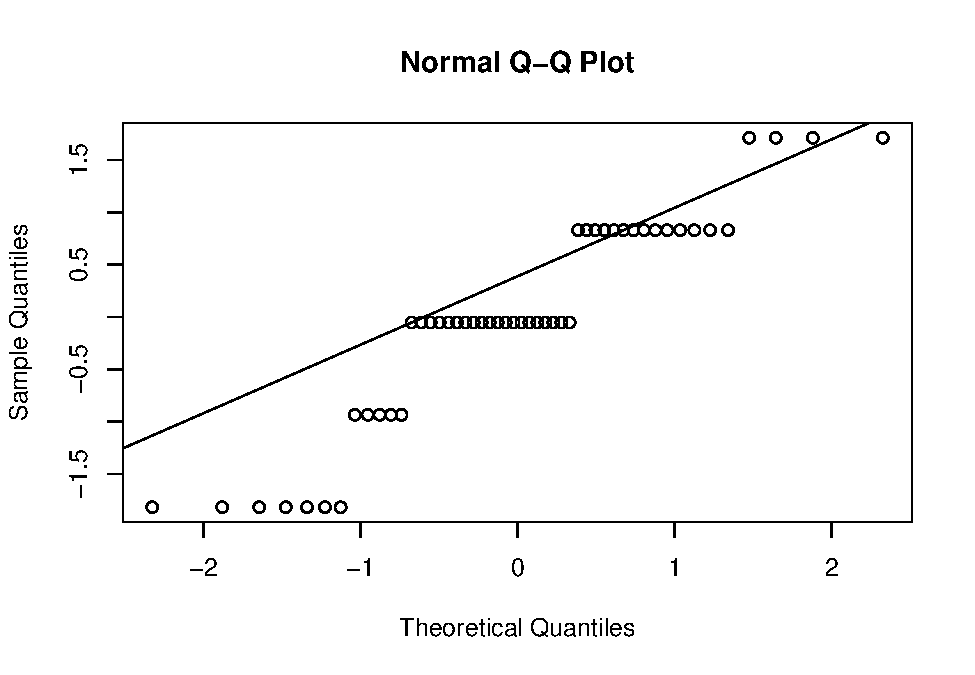
\includegraphics{01-intro_files/figure-latex/unnamed-chunk-4-1.pdf}

\hypertarget{statistical-inference}{%
\section{Statistical Inference}\label{statistical-inference}}

Summarizing data sets is important because no one can make sense of more than a few numbers at a time. But, data summaries cannot by themselves answer our research questions. That is because data summaries only say something about the particular data set we observe, while our research questions concern the whole population. Recall, a major aim of experimentation is generalizing from observations to population. When we make such generalizations we often refer to them as \emph{inferences}; and, statistical inferences are characterized by their careful treatment of statistical concepts, such as hypotheses, and Type 1 and 2 errors, which we discuss below.

A hypothesis is a claim or assertion about a population. These may be simple, i.e., ``the population mean is 5'', or more complex, like ``the population distribution of values is equivalent to a Normal probability distribution''. Notice that both of these statements are either true or false, yes or no. A hypothesis then may be called the ``null hypothesis'', and its complement (opposite) the alternative hypothesis. Which is which depends on the context. We make educated guesses about the truthfulness of a null hypothesis based on observations/data. Our educated guesses may be right or wrong, but we will never know because we will never ``see'' the whole population. If we reject the null hypothesis as false when it really is true, then we make a Type 1 error. The opposite, keeping the null hypothesis in favor over its alternative, when it is actually false, is a Type 2 error. Ideally, we would make no errors, but that's not possible. In fact, the two errors have an inverse relation. For example, if we adopt the rule that we always reject the null hypothesis, then we will necessarily maximize Type 1 errors but have no Type 2 errors. And, if we take the opposite approach, then we maximize Type 2 errors while making no Type 1 errors.

Much of this course will focus on constructing tests of relevant hypotheses with the property that we limit the chance of making a Type 1 error. By chance we refer to the probability distribution of the test outcome induced by random sampling of data from the population. A test that has chance no more than \(\alpha\) of making a Type 1 error is called a ``level \(\alpha\) test of \(H_0\)'', the null hypothesis.

\hypertarget{review-of-statistical-inference}{%
\chapter{Review of Statistical Inference}\label{review-of-statistical-inference}}

In this section we briefly review methods for constructing hypothesis tests. To keep things fairly simple, consider measuring one variable and suppose we obtain a simple random sample of such measurements/observations, denoted \(x_1, \ldots, x_n\). We'll refer to the random variable versions (yet to be observed versions) of such observations by \(X_1, \ldots, X_n\), per usual.

First we discuss the pivotal method for statistical inference, including approximate and asymptotic pivots. Next we'll briefly describe the bootstrap method, which, unlike the pivotal method, does not require a full sampling model of the data. Finally, we consider so-called ``randomization tests'' which are not exactly hypothesis tests, but provide a means for assessing whether interventions or observed differences are associated with significant response differences in both experiments and observational studies.

In terms of setup, suppose \(X^n := (X_1, \ldots, X_n)\) is a random sample of size \(n\) from a population equivalent to a probability distribution \(P\), and that we are interested in making inferences about a parameter \(\theta = \theta(P)\), a functional of \(P\). We'll consider special cases below. Also, for now we will consider only a ``point null'' hypothesis, \(H_0: \theta = \theta_0\) versus \(H_a:\theta \ne \theta_0\) where \(\theta_0\) is a singleton.

\hypertarget{pivotal-inference}{%
\section{Pivotal Inference}\label{pivotal-inference}}

Suppose \(H_0:\theta = \theta_0\). A pivot with respect to \(H_0\) is a function, say, \(g\), of data and parameter with a distribution \(F\) under \(H_0\) depending on no unknown parameters. We can write this relationship as
\[g(X_1, \ldots, X_n;\theta_0)\stackrel{H_0}\sim F.\]

You are likely familiar with several examples of pivots. If \(X^n\) is a random sample from a normal distribution with mean \(\mu\) and variance \(\sigma^2\), i.e., \(X_i\stackrel{iid}{\sim}N(\mu, \sigma^2), \,i=1,\ldots, n\), then
\[g(X^n;\mu):=\frac{\overline X - \mu}{\sqrt{S^2/n}}\stackrel{d}{=}t_{n-1}\]
where \(S^2\) is the sample variance of \(X^n\) and \(t_{n-1}\) is a Student's \(t\) random variable with \(n-1\) degrees of freedom.

A pivot for a point-null hypothesis admits a level-\(\alpha\) test by the following general rule:
\[\text{Reject }H_0\text{ if }g(x^n;\theta_0)\notin(U_{\alpha/2}, \, U_{1-\alpha/2})\]
where \(U\sim F\) and \(U_\alpha\) denotes the \(\alpha\) quantile of \(U\). The logic is as follows: if \(g(x^n;\theta_0)\notin(U_{\alpha/2}, \, U_{1-\alpha/2})\) then either \(g(x^n;\theta_0)\) is an unlikely realization of \(g(X^n;\theta_0)\) or \(H_0\) is false. Concluding \(H_0\) false in such an event is erroneous with probability
\[P_{H_0}(g(X^n;\theta_0)\leq U_{\alpha/2}) + P_{H_0}(g(X^n;\theta_0)\geq U_{1-\alpha/2}) = \alpha/2 + \alpha/2 = \alpha\]
by design. In the case of the normal random sample and point-null regarding \(\mu\) the general rule gives way to the \emph{one-sample t-test}
\[\text{Reject }H_0\text{ if }\frac{\overline X - \mu}{\sqrt{S^2/n}}\notin(t_{n-1, \alpha/2}, \, t_{n-1, 1-\alpha/2})\]

Pivot-based tests for point nulls have a one-to-one correspondence with \emph{confidence intervals}. Given data \(X^n = x^n\) define the confidence set \(C_{\alpha}(x^n):=\{\theta: g(x^n;\theta)\in(U_{\alpha/2}, \, U_{1-\alpha/2})\}\). The \emph{coverage probability} of \(C_\alpha(x^n)\) is equal to
\[P_{\theta_0}(\theta_0 \in C_\alpha(X^n))\]
where \(\theta_0\) is the true parameter value, i.e., in a point-null hypothesis test it is the null value and \(P_{\theta_0}\) means the same as \(P_{H_0}\).\\
\begin{align*} 
P_{\theta_0}(\theta_0 \in C_\alpha(X^n)) &= 1-P_{\theta_0}(\theta_0 \notin C_\alpha(X^n))\\
& = P_{\theta_0}(g(X^n;\theta_0)\notin(U_{\alpha/2}, \, U_{1-\alpha/2}))\\
& = 1-\alpha.
\end{align*}
Therefore, the confidence set given above (which is usually an interval) has the \emph{confidence property}
\[P_{\theta_0}(\theta_0 \in C_\alpha(X^n))\geq 1-\alpha.\]
Therefore, level-\(\alpha\) tests of point null hypotheses enjoy a one-to-one correspondence with valid/exact confidence sets (these being adjectives to describe sets with the confidence property).

\hypertarget{approximate-pivots}{%
\section{Approximate Pivots}\label{approximate-pivots}}

Introductory statistics courses often give students the impression pivots are common, and available in most problems. Rather, pivots are the exception, and pivot-based tests, for a variety of reasons, are simply the only tests covered in such courses. An early exception to the perceived rule is the two-sample t-test when population variances are unequal. Let's briefly entertain this slightly more complicated example involving two populations and two random samples, \(X^n\) and \(Y^m\) where \(X_i\stackrel{iid}{\sim}N(\mu_x, \sigma_x^2)\) and \(Y_j\stackrel{iid}{\sim}N(\mu_y, \sigma_y^2)\). As always, we want to test \(H_0:\mu_x-\mu_y = 0\), and a near-pivot is the expression
\[\frac{\overline X - \overline Y}{\sqrt{S_x^2/n + S_y^2/m}}.\]
We can rewrite this as
\[\frac{\overline X - \overline Y}{\sqrt{\sigma_x^2/n + \sigma_y^2/m}} \times \left[\frac{\sqrt{S_x^2/n + S_y^2/m}}{\sqrt{\sigma_x^2/n + \sigma_y^2/m}}\right]^{-1}.\]
Under \(H_0\), \(\frac{\overline X - \overline Y}{\sqrt{\sigma_x^2/n + \sigma_y^2/m}}\) has a standard normal distribution and \(S_x^2/n + S_y^2/m\) is equal in distribution to \(\sigma_x^2 V_{n-1} /[n(n-1)] + \sigma_y^2 U_{m-1} /[m(m-1)]\) where \(V_{n-1}\) and \(U_{m-1}\) are independent \(\chi^2\) r.v.'s with \(n-1\) and \(m-1\) degrees of freedom, respectively. The problem is that the denominator term in brackets is not equal in distribution to the square root of a \(\chi^2\) r.v. divided by its degrees of freedom. To get around this inconvenience, Satterthwaite suggested the following: find a \(\chi^2\) random variable \(R\) such that
\[\left[\frac{\sigma_x^2 V}{n(n-1)} + \frac{\sigma_y^2 U}{m(m-1)}\right]\cdot \left[\frac{\sigma_x^2}{n} + \frac{\sigma_y^2}{m}\right]^{-1}\stackrel{d}{\approx} R.\]
Satterthwaite's strategy for finding \(R\) was to choose the degrees of freedom of \(R\), denote \(\nu\) such that the mean of \(R\) and the variance of \(R\) match the mean and variance of the above expression. Let this degrees of freedom be \(\nu\) and note:
\[\nu = \left(\frac{s_x^2}{n} + \frac{s_y^2}{m}\right)^2\left[\frac{s_x^4}{n^2(n-1)}+\frac{s_y^4}{m^2(m-1)}\right]^{-1}.\]
Then, Sattethwaite showed
\[\frac{\overline X - \overline Y}{\sqrt{S_x^2/n + S_y^2/m}}\stackrel{d}{\approx} R_\nu,\]
which is the approximate pivot used in the two-sample t-test when the variances are not assumed equal.

It is often the case that tests based on approximate pivots are not level-\(\alpha\) tests, but depending on the case some, like the two-sample t-test, perform very well with respect to nominal Type 1 error. Just to be clear, we'll define an approximate pivot as a function of statistics and parameters approximated by a known distribution:
\[g(X^n; \theta_0)\stackrel{\cdot}{\sim} F, \quad \text{under }H_0\]
where the dot above the tilde denotes ``approximately follows distribution function \(F\)''. A special case of an approximate pivot is one whose approximation improves as the sample size \(n\) increases---we call these asymptotic pivots as we discuss next.

\hypertarget{asymptotic-pivots-and-likelihood-based-tests}{%
\section{Asymptotic Pivots and Likelihood-based Tests}\label{asymptotic-pivots-and-likelihood-based-tests}}

Define an asymptotic pivot as follows:
\[g(X^n; \theta_0)\stackrel{d}{\rightarrow} F, \quad \text{under }H_0, \, \text{as }n\rightarrow\infty.\]
This simply says that the distribution function of \(g(X^n; \theta_0)\) converges to \(F\) as \(n\rightarrow \infty\) when \(H_0\) is true. For ``large'' \(n\) we would expect a test based on this asymptotic pivot to be nearly a level-\(\alpha\) test---but sometimes it may be difficult to determine what values of \(n\) are sufficiently large for this good behavior to ``kick in''.

Here's an asymptotic-pivot based test you've hear of: consider the one-sample t-test that rejects \(H_0:\mu = \mu_0\) when \((\overline x - \mu_0)/\sqrt{s^n/n} \notin (t_{n-1,\alpha/2}, t_{n-1,1-\alpha/2})\). Now, replace the Student's \(t\) quantiles with standard normal quantiles. Since \(t_{n-1}\stackrel{d}{\rightarrow}N(0,1)\) as \(n\rightarrow \infty\), the ``z-test'' is approximately a level-\(\alpha\) test for ``large'' \(n\), usually \(n>50\) is plenty.

Fortunately, there is a powerful way to derive asymptotic pivots in a wide variety of situations using maximum likelihood. For review, recall the likelihood function for a random sample is
\[L(\theta;x^n) = \prod_{i=1}^n f(x_i;\theta)\]
where \(f(x;\theta)\) denotes the density of \(X\). The loglikelihood is simply \(\ell(\theta;x^n) = \log(L(\theta;x^n))\) where log always denotes the natural log. The maximum likelihood estimator \(\hat\theta_{mle}\) is the (usually unique) value \(\hat\theta_{mle} = \arg\min \ell(\theta;x^n)\). Also, recall the Fisher information (for one sample) is given by \(I(\theta) = -E(\frac{\partial^2}{\partial\theta^2}\ell(\theta;X^n))\). Then, the following is an asymptotic pivot:
\[n^{1/2}\sqrt{I(\hat\theta_{mle})}(\hat\theta_{mle} - \theta_0)\stackrel{d}{\rightarrow}N(0,1).\]
Tests based on such a pivot are called asymptotic Wald tests. There are other ways of constructing likelihood-based tests, such as likelihood ratio tests and score-based tests. But, we will not discuss those here.

\hypertarget{bootstrap-based-tests}{%
\section{Bootstrap-based Tests}\label{bootstrap-based-tests}}

The \emph{bootstrap} (and related jackknife) are a collection of techniques for statistical inference that (usually) do not require one to specify the sampling distribution of the data. For example, consider inference on the population median, \(\theta\). Regardless of \(P\), the median satisfies \(\theta = \theta(P) = \text{argsolve}\left\{0.5=\int_{-\infty}^\theta dP\right\}\). The median always exists, independently of the sampling distribution \(P\); so, the concept of inference on \(\theta\) is sensible whether anything about \(P\) is known or not. Should we choose some particular form of \(P\), say, normal, when in fact \(P\) is not normal, then we are likely to make poor (biased) inferences regarding \(\theta\). It behooves us not to \emph{misspecify} \(P\). But, then we need statistical inference techniques that do not require specifying \(P\). Enter the bootstrap.

The bootstrap typically centers around a point estimator. Carrying on the median example, let \(\hat\theta\) denote the sample median with respect to \(x^n\). The bootstrap instructs us to generate \emph{resamples} of \(x^n\) by sampling from \(x^n\) with replacement, \(n\) times, and repeat this process \(B\) times, generating the \emph{bootstrapped} data sets \(x^{n,1}, x^{n,2}, \ldots, x^{n,B}\). An illustration of this is given below for \(n=10\) and \(B = 5\); typically, \(B\) is very large.

\begin{Shaded}
\begin{Highlighting}[]
\NormalTok{x }\OtherTok{\textless{}{-}} \FunctionTok{rnorm}\NormalTok{(}\DecValTok{10}\NormalTok{)}
\FunctionTok{print}\NormalTok{(}\StringTok{\textquotesingle{}original data\textquotesingle{}}\NormalTok{)}
\end{Highlighting}
\end{Shaded}

\begin{verbatim}
## [1] "original data"
\end{verbatim}

\begin{Shaded}
\begin{Highlighting}[]
\FunctionTok{print}\NormalTok{(}\FunctionTok{sort}\NormalTok{(}\FunctionTok{round}\NormalTok{(x,}\DecValTok{2}\NormalTok{)))}
\end{Highlighting}
\end{Shaded}

\begin{verbatim}
##  [1] -1.13 -1.02 -0.49 -0.43  0.33  0.67  0.83  1.13  1.34  1.57
\end{verbatim}

\begin{Shaded}
\begin{Highlighting}[]
\FunctionTok{print}\NormalTok{(}\StringTok{\textquotesingle{}bootstrapped data sets\textquotesingle{}}\NormalTok{)}
\end{Highlighting}
\end{Shaded}

\begin{verbatim}
## [1] "bootstrapped data sets"
\end{verbatim}

\begin{Shaded}
\begin{Highlighting}[]
\ControlFlowTok{for}\NormalTok{(i }\ControlFlowTok{in} \DecValTok{1}\SpecialCharTok{:}\DecValTok{5}\NormalTok{)\{}
\NormalTok{ y }\OtherTok{=} \FunctionTok{sample}\NormalTok{(}\FunctionTok{round}\NormalTok{(x,}\DecValTok{2}\NormalTok{),}\DecValTok{10}\NormalTok{,}\AttributeTok{replace =} \ConstantTok{TRUE}\NormalTok{)}
 \FunctionTok{print}\NormalTok{(}\FunctionTok{sort}\NormalTok{(y))}
\NormalTok{\}}
\end{Highlighting}
\end{Shaded}

\begin{verbatim}
##  [1] -1.13 -1.13 -1.02 -0.49 -0.43 -0.43  0.33  0.67  0.83  0.83
##  [1] -0.49 -0.43  0.33  0.33  0.33  0.67  0.67  0.83  1.13  1.57
##  [1] -1.13 -0.49 -0.49 -0.49 -0.49 -0.43 -0.43  0.67  1.13  1.13
##  [1] -1.13 -0.43 -0.43  0.33  0.67  0.67  1.13  1.34  1.34  1.34
##  [1] -1.13 -1.02 -0.49 -0.43 -0.43 -0.43  0.83  1.57  1.57  1.57
\end{verbatim}

For each bootstrapped data set, we compute its corresponding point estimator, in this case the sample median, and call it \(\hat\theta^b\) for \(b = 1, \ldots, B\). These represent a sample of size \(B\) from the bootstrap sampling distribution of the point estimator. For large \(n\) and \(B\), and under certain other conditions, the bootstrap sampling distribution of \(\hat\theta\) is a very good approximation of the true sampling distribution of \(\hat\theta\), which is unknown because \(P\) is unknown. See a histogram of \(1000\) bootstrapped sample medians based on an original sample of \(n=10\) from a standard normal population.

\begin{Shaded}
\begin{Highlighting}[]
\FunctionTok{library}\NormalTok{(boot)}
\NormalTok{x }\OtherTok{\textless{}{-}} \FunctionTok{rnorm}\NormalTok{(}\DecValTok{10}\NormalTok{)}
\NormalTok{fun }\OtherTok{=} \ControlFlowTok{function}\NormalTok{(data, i)\{}
  \FunctionTok{return}\NormalTok{(}\FunctionTok{median}\NormalTok{(data[i]))}
\NormalTok{\}}
\NormalTok{booted.medians }\OtherTok{\textless{}{-}} \FunctionTok{boot}\NormalTok{(}\AttributeTok{data =}\NormalTok{ x, }\AttributeTok{statistic =}\NormalTok{ fun, }\AttributeTok{R =} \DecValTok{1000}\NormalTok{, }\AttributeTok{stype =} \StringTok{\textquotesingle{}i\textquotesingle{}}\NormalTok{)}
\FunctionTok{hist}\NormalTok{(booted.medians}\SpecialCharTok{$}\NormalTok{t, }\AttributeTok{xlab =} \StringTok{\textquotesingle{}Bootstrapped sample medians\textquotesingle{}}\NormalTok{, }\AttributeTok{main =} \StringTok{\textquotesingle{}\textquotesingle{}}\NormalTok{)}
\end{Highlighting}
\end{Shaded}

\includegraphics{02-Review_of_Inference_files/figure-latex/unnamed-chunk-2-1.pdf}

Given the bootstrap sampling distribution of \(\hat\theta\), sall it \(\hat F\), there are many ways to proceed with inference on \(\theta\). The most straightforward method is to treat the extreme quantiles of \(\hat F\) as implausible values of \(\theta\). Let \(\hat\theta_\alpha\) denote the \(\alpha\) quantile of the bootstrap sampling distribution of \(\hat\theta\). Then, \((\hat\theta_{\alpha/2}, \,\hat\theta_{1-\alpha/2})\) constitutes an approximate \(95\%\) bootstrap CI for \(\theta\), and, similarly, the complement of that set is a rejection region for the point null \(H_0:\theta = \theta_0\). These quantiles are estimated by the corresponding sample quantiles of the \(\hat\theta^b\) values. This is called the \emph{percentile bootstrap method}. For various reason we will not discuss here, a different method is usually preferred for deriving bootstrap CIs and tests. Let \(\hat\theta_\alpha\) denote the \(\alpha\) quantile of the bootstrap sampling distribution of \(\hat\theta\). Let \(\overline \theta\) denote the bootstrap sample mean \(B^{-1}\sum_{b=1}^B \hat\theta^b\). Then, \((2\overline \theta - \hat\theta_{1-\alpha/2}, \,2\overline \theta - \hat\theta_{\alpha/2})\) is the so-called \emph{basic bootstrap CI} for \(\theta\). Again, its complement set may be used as a rejection region for a point null.

Many other bootstrap techniques are available for different resampling schemes, different constructions of intervals and tests, and different assumptions regarding the sampling distribution. The basic message to keep in mind is that the bootstrap is a general-purpose method with wide applicability, like mle, but for use when the sampling distribution is totally unknown.

\hypertarget{randomization-and-permutation-tests}{%
\section{Randomization and Permutation Tests}\label{randomization-and-permutation-tests}}

We finish our general discussion of constructing tests and confidence intervals with randomization tests, which is a bit of a misnomer. In fact, these are not really tests at all. As defined above, tests concern evaluating statements about the population, which involves generalizing from the sample to the population. Randomization tests attempt to evaluate whether an intervention or observed characteristic is responsible for observed differences in responses \textbf{within the observed data set}. The following illustration helps to clarify the difference between hypothesis tests and randomization tests.

Suppose \(x^n\) is an observed random sample from a population. Let \(y^n \in \{0,1\}^n\) denote a binary grouping variable identifying the observations in \(x^n\) with one of two groups. For a concrete example, we can think of \(y^n\) indicating a randomized treatment with one of two drugs, and \(x^n\) recording an outcome, like reduction in blood pressure after treatment for patients with high blood pressure. A hypothesis about the population may claim something like ``there is no difference in average reduction in blood pressure between the two drugs at the population level''. Of course, this data set would be relevant for evaluating such a hypothesis. A subtly different claim is the following: ``the observed difference in mean blood pressure reduction is not attributable to which treatment/drug was received''. The latter is a claim only about the observed treatment effects, and not the population-level effects. A randomization test is used to evaluate this second type of claim.

To perform a randomization test, one simply permutes the values in \(y^n\)---which, if the claim is true, is simply equivalent to the randomization of patients into the two treatment groups having come out differently than observed---and re-compute the difference of sample means. Of course, now we have jumbled up the responses of patients in the two treatment groups, but that's the point. The claim is that the effects of the two treatments are indistinguishable, and so it shouldn't matter if we re-label/re-randomize the patients. If we repeat these two steps many, many times (similar to the bootstrap) we obtain a \emph{randomization distribution} or \emph{permutation distribution} of the difference of sample means. To evaluate the claim, similar to the bootstrap, we simply look at the extreme quantiles of this distribution and see if they contain the observed difference in sample means. If so, then the observed difference is a value typical of the distribution that we realized under the assumption that the treatment labels were exchangeable, and, hence, the claim of no difference is reasonable. On the other hand, if the observed difference in means is outside the randomization distribution, then it is implausible that the treatment labels are not associated with the observed difference. The example below shows the randomization difference as well as the observed difference for randomly generated data sets of size ten from two normal distributions, \(N(0,1)\) and \(N(1,2)\). The blue points show the middle \(95\%\) of re-randomized differences of sample means and the vertical line shows the observed difference.

\begin{Shaded}
\begin{Highlighting}[]
\FunctionTok{set.seed}\NormalTok{(}\DecValTok{12345}\NormalTok{)}
\NormalTok{x }\OtherTok{\textless{}{-}} \FunctionTok{rnorm}\NormalTok{(}\DecValTok{10}\NormalTok{)}
\NormalTok{y }\OtherTok{\textless{}{-}} \FunctionTok{rnorm}\NormalTok{(}\DecValTok{10}\NormalTok{,}\DecValTok{1}\NormalTok{,}\DecValTok{2}\NormalTok{)}
\NormalTok{z }\OtherTok{\textless{}{-}} \FunctionTok{mean}\NormalTok{(x) }\SpecialCharTok{{-}} \FunctionTok{mean}\NormalTok{(y)}
\NormalTok{rerandomize }\OtherTok{\textless{}{-}} \ControlFlowTok{function}\NormalTok{(B)\{}
\NormalTok{  data }\OtherTok{\textless{}{-}} \FunctionTok{c}\NormalTok{(x,y)}
\NormalTok{  zs }\OtherTok{\textless{}{-}} \FunctionTok{rep}\NormalTok{(}\ConstantTok{NA}\NormalTok{,B)}
  \ControlFlowTok{for}\NormalTok{(i }\ControlFlowTok{in} \DecValTok{1}\SpecialCharTok{:}\NormalTok{B)\{}
\NormalTok{    indices }\OtherTok{\textless{}{-}} \FunctionTok{sample}\NormalTok{(}\DecValTok{1}\SpecialCharTok{:}\DecValTok{20}\NormalTok{, }\DecValTok{10}\NormalTok{, }\AttributeTok{replace =} \ConstantTok{FALSE}\NormalTok{)}
\NormalTok{    new.x }\OtherTok{\textless{}{-}}\NormalTok{ data[indices]}
\NormalTok{    new.y }\OtherTok{\textless{}{-}}\NormalTok{ data[}\SpecialCharTok{{-}}\NormalTok{indices]}
\NormalTok{    new.z }\OtherTok{\textless{}{-}} \FunctionTok{mean}\NormalTok{(new.x) }\SpecialCharTok{{-}} \FunctionTok{mean}\NormalTok{(new.y)}
\NormalTok{    zs[i] }\OtherTok{\textless{}{-}}\NormalTok{ new.z}
\NormalTok{  \}}
\FunctionTok{return}\NormalTok{(zs)}
\NormalTok{\}}
\NormalTok{zs }\OtherTok{\textless{}{-}} \FunctionTok{rerandomize}\NormalTok{(}\DecValTok{1000}\NormalTok{)}
\FunctionTok{hist}\NormalTok{(zs, }\AttributeTok{main =} \StringTok{\textquotesingle{}\textquotesingle{}}\NormalTok{, }\AttributeTok{xlab =} \StringTok{\textquotesingle{}re{-}randomized differences of group sample means\textquotesingle{}}\NormalTok{)}
\FunctionTok{abline}\NormalTok{(}\AttributeTok{v =}\NormalTok{ z)}
\FunctionTok{quantile}\NormalTok{(zs, }\FunctionTok{c}\NormalTok{(}\FloatTok{0.025}\NormalTok{,}\FloatTok{0.975}\NormalTok{))  }
\end{Highlighting}
\end{Shaded}

\begin{verbatim}
##      2.5%     97.5% 
## -1.301027  1.400158
\end{verbatim}

\begin{Shaded}
\begin{Highlighting}[]
\NormalTok{z  }
\end{Highlighting}
\end{Shaded}

\begin{verbatim}
## [1] -1.7049
\end{verbatim}

\begin{Shaded}
\begin{Highlighting}[]
\FunctionTok{points}\NormalTok{(}\FunctionTok{c}\NormalTok{(}\FunctionTok{quantile}\NormalTok{(zs, }\FunctionTok{c}\NormalTok{(}\FloatTok{0.025}\NormalTok{,}\FloatTok{0.975}\NormalTok{))), }\FunctionTok{c}\NormalTok{(}\DecValTok{0}\NormalTok{,}\DecValTok{0}\NormalTok{), }\AttributeTok{pch =} \DecValTok{19}\NormalTok{, }\AttributeTok{col =} \StringTok{\textquotesingle{}blue\textquotesingle{}}\NormalTok{)}
\end{Highlighting}
\end{Shaded}

\includegraphics{02-Review_of_Inference_files/figure-latex/unnamed-chunk-3-1.pdf}

As hinted above, randomization tests are often performed on data from observational studies, where the grouping variables does not represent an intervention. A common example is evaluating male/female differences. In this context the same test is usually called a permutation test, because the relation to randomization of an intervention over subjects is lost, but the idea of permuting class labels is the same.

Finally, we describe the construction of (something like) confidence intervals from randomization/permutation tests. If we keep the correspondence, i.e., that the confidence interval is simply the set of point null values for which the point null is not rejected at level \(\alpha\), then it turns out to be fairly complicated to obtain the interval, at least numerically speaking. Before going further, note that the use of the phrase ``point null'' is rather loose here. The null hypothesis of no difference described above is specifically in relation to the observed data set, i.e., that the labeling is not associated with a response difference in the observed data. It's not really a hypothesis in the sense of a claim about the population; rather, it's a claim about the sample. Now, to obtain an interval of ``plausible'' values of differences, we have to amend our statement. Let's say that the effect of labeling is a difference of \(\theta\) in the observed data, with respect to the group 1 minus group 0 comparison. To evaluate this claim we would subtract \(\theta\) from every response with an original label of 1, the idea being that we have then removed the overall effect of labeling. Then, we perform the randomization test as before for the data set with \(\theta\) subtracted from the first group's responses, comparing the randomization distribution of this difference to the realized value. We have to repeat the randomization test over a range of \(\theta\) values, recording which are rejected and which are not. In this manner we can build an interval from the smallest to the largest \(\theta\) values not rejected by the randomization test procedure. Be careful implementing this procedure as it can take a good deal of time!

\begin{Shaded}
\begin{Highlighting}[]
\FunctionTok{set.seed}\NormalTok{(}\DecValTok{12345}\NormalTok{)}
\NormalTok{x }\OtherTok{\textless{}{-}} \FunctionTok{rnorm}\NormalTok{(}\DecValTok{10}\NormalTok{)}
\NormalTok{y }\OtherTok{\textless{}{-}} \FunctionTok{rnorm}\NormalTok{(}\DecValTok{10}\NormalTok{,}\DecValTok{1}\NormalTok{,}\DecValTok{2}\NormalTok{)}
\NormalTok{z }\OtherTok{\textless{}{-}} \FunctionTok{mean}\NormalTok{(x) }\SpecialCharTok{{-}} \FunctionTok{mean}\NormalTok{(y)}
\NormalTok{theta.seq }\OtherTok{\textless{}{-}} \FunctionTok{seq}\NormalTok{(}\AttributeTok{from =} \SpecialCharTok{{-}}\DecValTok{4}\NormalTok{, }\AttributeTok{to =} \DecValTok{4}\NormalTok{, }\AttributeTok{length.out =} \DecValTok{100}\NormalTok{)}
\NormalTok{rejects}\OtherTok{\textless{}{-}} \FunctionTok{rep}\NormalTok{(}\ConstantTok{NA}\NormalTok{,}\FunctionTok{length}\NormalTok{(theta.seq))}
\NormalTok{z.h0 }\OtherTok{\textless{}{-}}\NormalTok{ rejects}
\NormalTok{rerandomize }\OtherTok{\textless{}{-}} \ControlFlowTok{function}\NormalTok{(B, theta)\{}
\NormalTok{  data }\OtherTok{\textless{}{-}} \FunctionTok{c}\NormalTok{(x}\SpecialCharTok{{-}}\NormalTok{theta,y)}
\NormalTok{  zs }\OtherTok{\textless{}{-}} \FunctionTok{rep}\NormalTok{(}\ConstantTok{NA}\NormalTok{,B)}
  \ControlFlowTok{for}\NormalTok{(i }\ControlFlowTok{in} \DecValTok{1}\SpecialCharTok{:}\NormalTok{B)\{}
\NormalTok{    indices }\OtherTok{\textless{}{-}} \FunctionTok{sample}\NormalTok{(}\DecValTok{1}\SpecialCharTok{:}\DecValTok{20}\NormalTok{, }\DecValTok{10}\NormalTok{, }\AttributeTok{replace =} \ConstantTok{FALSE}\NormalTok{)}
\NormalTok{    new.x }\OtherTok{\textless{}{-}}\NormalTok{ data[indices]}
\NormalTok{    new.y }\OtherTok{\textless{}{-}}\NormalTok{ data[}\SpecialCharTok{{-}}\NormalTok{indices]}
\NormalTok{    new.z }\OtherTok{\textless{}{-}} \FunctionTok{mean}\NormalTok{(new.x) }\SpecialCharTok{{-}} \FunctionTok{mean}\NormalTok{(new.y)}
\NormalTok{    zs[i] }\OtherTok{\textless{}{-}}\NormalTok{ new.z}
\NormalTok{  \}}
\FunctionTok{return}\NormalTok{(zs)}
\NormalTok{\}}
\ControlFlowTok{for}\NormalTok{(j }\ControlFlowTok{in} \DecValTok{1}\SpecialCharTok{:}\FunctionTok{length}\NormalTok{(theta.seq))\{}
\NormalTok{  z.h0[j] }\OtherTok{=} \FunctionTok{mean}\NormalTok{(x) }\SpecialCharTok{{-}}\NormalTok{ theta.seq[j] }\SpecialCharTok{{-}} \FunctionTok{mean}\NormalTok{(y)}
\NormalTok{  zs }\OtherTok{\textless{}{-}} \FunctionTok{rerandomize}\NormalTok{(}\DecValTok{1000}\NormalTok{, theta.seq[j])}
\NormalTok{  qzs }\OtherTok{\textless{}{-}} \FunctionTok{quantile}\NormalTok{(zs, }\FunctionTok{c}\NormalTok{(}\FloatTok{0.025}\NormalTok{,}\FloatTok{0.975}\NormalTok{))  }
\NormalTok{  rejects[j] }\OtherTok{\textless{}{-}} \FunctionTok{ifelse}\NormalTok{(z.h0[j] }\SpecialCharTok{\textless{}}\NormalTok{ qzs[}\DecValTok{1}\NormalTok{] }\SpecialCharTok{||}\NormalTok{ z.h0[j] }\SpecialCharTok{\textgreater{}}\NormalTok{ qzs[}\DecValTok{2}\NormalTok{], }\DecValTok{1}\NormalTok{, }\DecValTok{0}\NormalTok{)}
\NormalTok{\}}
\FunctionTok{c}\NormalTok{(}\FunctionTok{min}\NormalTok{(theta.seq[rejects}\SpecialCharTok{==}\DecValTok{0}\NormalTok{]), }\FunctionTok{max}\NormalTok{(theta.seq[rejects}\SpecialCharTok{==}\DecValTok{0}\NormalTok{]))}
\end{Highlighting}
\end{Shaded}

\begin{verbatim}
## [1] -2.8686869 -0.5252525
\end{verbatim}

\hypertarget{exercises}{%
\section{Exercises}\label{exercises}}

\begin{enumerate}
\def\labelenumi{\arabic{enumi}.}
\item
  Verify the Welch-Satterthwaite degrees of freedom for the two-sample t-test by Satterthwaite's method of moments as describes above.
\item
  Recall that a level-\(\alpha\) test must limit Type 1 error probability to no more than \(\alpha\%\), not necessarily reach exactly \(\alpha\%\), although equality is better (otherwise the test is conservative). reconsider the two-sample t-test. Hsu and Scheffe showed that a (conservative) level-\(\alpha\) test is based on the approximate pivot
  \[\frac{\overline X - \overline Y}{\sqrt{S_x^2/n + S_y^2/m}}\leq_{st} t_m\]
  where \(m:=\min\{n-1, m-1\}\), \(t_m\) is a Student's \(t\) r.v. with \(m\) df, and \(X\leq_{st} Y\) means \(X\) is stochastically smaller than \(Y\). If you're not familiar with the term, \(X\) is stochastically smaller than \(Y\) if \(P(X>s)\leq P(Y>s)\) for \(s\in \mathbb{R}\). In other words, the \(t_m\) distribution has heavier tails than the approximate pivotal quantity, which explains why the test is conservative.
\end{enumerate}

Do either of the following:

\begin{itemize}
\tightlist
\item
  Implement a Monte Carlo simulation to verify the claim that Hsu and Scheffe's test is valid, albeit conservative.
\item
  Verify the claim analytically.
\end{itemize}

\begin{enumerate}
\def\labelenumi{\arabic{enumi}.}
\setcounter{enumi}{2}
\item
  Let \(X^n\) denote a random sample of size \(n\) from and exponential distribution with rate parameter \(\lambda\). Find the mle, the Fisher information, and a \(95\%\) CI for \(\lambda\) based on the asymptotic Wald test.
\item
  Let \(X^n\) denote a random sample of size \(n\) from a normal distribution with mean \(\mu\) and variance \(\sigma^2\). Find the mle of \((\mu, \sigma^2)\); recall this is the vector of values such that the gradient of the (log)likelihood is zero. Find the Fisher information matrix for \((\mu, \sigma^3)\); recall this is minus one times the expectation of the second derivative matrix of the loglikelihood. And, finally, find a \(95\%\) CI for \(\mu\) based on the asymptotic Wald test. Hint: recall the marginal variance of \(\hat\mu_{mle}\) is the corresponding diagonal entry of the inverse of the Fisher information matrix.
\item
  Recall the delta method: let \(g(\theta)\) be a smooth function of a vector parameter. Then, the mle of \(g(\theta)\) is \(g(\hat\theta_{mle})\), and it has the following large sample normal behavior:
  \[n^{1/2}(g(\hat\theta_{mle})-g(\theta)) \stackrel{\cdot}{\sim} N(0, g'(\theta)^\top I(\theta)^{-1}g(\theta)).\]
  Use the delta method to find a \(95\%\) confidence interval for the signal-to-noise ratio \(\mu/\sigma\) based on a random sample \(X^n\) of size \(n\) from \(N(\mu, \sigma^2)\).
\item
  Besides the above delta method, you probably can't think of another way to construct a test or CI for the signal-to-noise ratio \(\eta:=\mu/\sigma\) of a normal population; certainly, you probably can't think of a pivot for such a quantity. Towards deriving a (non-asymptotic) level-\(\alpha\) test for \(H_0:\eta = \eta_0\) write down the following \emph{data-generating equations} in terms of the sufficient statistics \((\overline X, S^2)\):
  \begin{align*} 
  \overline X &= \mu + n^{-1/2}\sigma Z, \quad Z\sim N(0,1)\\
  (n-1)S^2 &= \sigma^2 V, \quad V\sim \chi^2(n-1), \quad V\perp Z.
  \end{align*}
  Make the one-to-one transformation \((\mu, \sigma^2)\mapsto(\eta, \sigma^2)\) and re-write the equations equivalently in terms of the new parametrization:
  \begin{align*} 
  \overline X &= \sigma \eta + n^{-1/2}\sigma Z, \quad Z\sim N(0,1)\\
  (n-1)S^2 &= \sigma^2 V, \quad V\sim \chi^2(n-1), \quad V\perp Z.
  \end{align*}
  Into the first equation, plug in \(\sigma = \sqrt{(n-1)S^2/V}\) to arrive at
  \begin{align*} 
  \overline X &= \eta\sqrt{(n-1)S^2/V} + n^{-1/2}\sqrt{(n-1)S^2/V} Z, \quad Z\sim N(0,1)\\
  (n-1)S^2 &= \sigma^2 V, \quad V\sim \chi^2(n-1), \quad V\perp Z.
  \end{align*}
  Now, make the following observation, keeping in mind we are only interested in \(\eta\), not \(\sigma^2\). Fix any values of \((\overline X, \eta, S^2, V, Z)\) such that the first equation is satisfied. It follows that there exists a value of \(\sigma^2>0\) simultaneously satisfying the second equation. Therefore, we can ignore the second equation. This is similar to what happens in the case of the one-sample t-test where we find a pivot not depending on \(\sigma^2\). Divide by \(\sqrt{S^2}\) on both sides of the first equation: we are left with the following:
  \[\frac{\overline X}{\sqrt{S^2}} = \sqrt{(n-1)/V}\left (\eta + n^{-1/2}Z\right), \quad Z\sim N(0,1)\quad V\sim \chi^2(n-1), \quad V\perp Z.\]
  If you stare at this equation long enough, you will convince yourself you cannot solve for a pivot. Nevertheless, we have something similar, namely, a single equation involving the parameter of interest, the sufficient statistics, and random variables with known distributions. Define the following function:
  \[\pi(\eta) = 1-\left|2P_{Z,V}\left(\frac{\overline x}{\sqrt{s^2}} \leq \sqrt{(n-1)/V}\left (\eta + n^{-1/2}Z\right)\right) - 1\right|.\]
  Claim: the test that rejects \(H_0:\eta= \eta_0\) when \(\pi(\eta_0) <\alpha\) is a level-alpha test. Similarly, the set \(\{\eta: \pi(\eta) > \alpha\}\) is a valid \((1-\alpha)\) confidence set.
\end{enumerate}

Do either one the following:

\begin{itemize}
\tightlist
\item
  Implement a Monte Carlo simulation to verify the claim.
\item
  Verify the claim analytically.
\end{itemize}

\hypertarget{introduction-to-linear-models}{%
\chapter{Introduction to Linear Models}\label{introduction-to-linear-models}}

In this section we define linear models, provide simple examples, and analyze linear models for one- and two-sample problems.

\hypertarget{defining-the-linear-model}{%
\section{Defining the linear model}\label{defining-the-linear-model}}

Every linear model defines a linear relationship between an independent variable \(Y\) and a dependent variable \(X\), including a random term \(\epsilon\):
\begin{equation}
Y = X\beta + \epsilon
  \label{eq:linmod}
\end{equation}
Usually, \(X\) is a fixed or non-random variable, while \(\epsilon\) is a random variable representing variation due to a random sampling mechanism, so that \(Y\) is a random outcome. Further, in \eqref{eq:linmod} \(Y = (Y_1, \ldots, Y_n)^\top\) is an \(n\times 1\) vector of outcomes/responses, \(X\) is an \(n\times p\) matrix of fixed variables/covariates (\(p<n\)), \(\epsilon = (\epsilon_1, \ldots, \epsilon_n)^\top\) is an \(n\times 1\) vector of random variables, and \(\beta = (\beta_1, \ldots, \beta_p)^{\top}\) is a \(p\times 1\) coefficient vector of unknown parameters.

The \emph{least-squares model} or just called the \emph{linear model} is the above model with few or no additional assumptions although, to estimate the unknown parameter \(\beta\), which characterizes the relationship between \(X\) and \(Y\), assuming \(E(\epsilon_i) = 0\) is very helpful and usually reasonable.

The \emph{Gauss-Markov model}---which we will tacitly use throughout the course and examine in detail at the end of the semester---makes the assumptions \(E(\epsilon_i) = 0\), \(E(\epsilon_i^2) = \sigma^2\), which means the ``error'' term \(\epsilon\) has the same variance for each random sample (homogeneous or constant variance), and \(E(\epsilon_i\epsilon_j)=0\). Or, in other words, the last two assumptions may be written \(Cov(\epsilon) = \sigma^2 I_{n}\) where \(I_n\) is the \(n\times n\) identity matrix.

\hypertarget{gauss-markov-model-for-one-sample}{%
\section{Gauss-Markov model for one-sample}\label{gauss-markov-model-for-one-sample}}

Let \(P\) be a normal population with mean \(\beta\) and variance \(\sigma^2\). Let \(Y_i\stackrel{iid}{\sim}P\). Then, we may write
\begin{equation}
\begin{aligned}
Y_i &= \beta x_i + \epsilon_i, \quad i = 1,\ldots, n, \,\,\text{or}\\
Y &= X\beta + \epsilon
\end{aligned}
\end{equation}
where \(x_i = 1\), so that \(X = (1, 1, ..., 1)^{\top}\) is an \(n\times 1\) vector of ones.

\hypertarget{blocks}{%
\chapter{Blocks}\label{blocks}}

\hypertarget{equations}{%
\section{Equations}\label{equations}}

Here is an equation.

\begin{equation} 
  f\left(k\right) = \binom{n}{k} p^k\left(1-p\right)^{n-k}
  \label{eq:binom}
\end{equation}

You may refer to using \texttt{\textbackslash{}@ref(eq:binom)}, like see Equation \eqref{eq:binom}.

\hypertarget{theorems-and-proofs}{%
\section{Theorems and proofs}\label{theorems-and-proofs}}

Labeled theorems can be referenced in text using \texttt{\textbackslash{}@ref(thm:tri)}, for example, check out this smart theorem \ref{thm:tri}.

\begin{theorem}
\protect\hypertarget{thm:tri}{}\label{thm:tri}For a right triangle, if \(c\) denotes the \emph{length} of the hypotenuse
and \(a\) and \(b\) denote the lengths of the \textbf{other} two sides, we have
\[a^2 + b^2 = c^2\]
\end{theorem}

Read more here \url{https://bookdown.org/yihui/bookdown/markdown-extensions-by-bookdown.html}.

\hypertarget{callout-blocks}{%
\section{Callout blocks}\label{callout-blocks}}

The R Markdown Cookbook provides more help on how to use custom blocks to design your own callouts: \url{https://bookdown.org/yihui/rmarkdown-cookbook/custom-blocks.html}

  \bibliography{book.bib,packages.bib}

\end{document}
